% \documentclass[../main.tex]{subfiles}

% \begin{document}

{
\setstretch{1.0}
\chapter{Bivalves as emerging model systems to study the mechanisms and evolution of sex determination: a genomic point of view}
\label{perspective}

\noindent{\large{Filippo Nicolini\textsuperscript{1,2}, Fabrizio Ghiselli\textsuperscript{1}, Andrea Luchetti\textsuperscript{1}, Liliana Milani\textsuperscript{1}}}

\vspace{5mm}

\noindent{\textsuperscript{1}\textit{Department of Biological, Geological and Environmental Science, University of Bologna, Bologna (BO), Italy}.}

\noindent{\textsuperscript{2}\textit{Fano Marine Center, Fano (PU), Italy}.}

\vspace{5mm}

\noindent{\textbf{Published in}: 2023, \textit{Genome Biology and Evolution}, 15(10):evad181. \hfill \\ \href{https://doi.org/10.1093/gbe/evad181}{10.1093/gbe/evad181}}
}

\vspace{5mm}

\textbf{Abstract}. Bivalves are a diverse group of molluscs that have recently attained a central role in plenty of biological research fields, thanks to their peculiar life history traits. Here we propose that bivalves should be considered as emerging model systems also in sex-determination studies, since they would allow to investigate: (i) the transition between environmental and genetic sex determination, with respect to different reproductive backgrounds and sexual systems (from species with strict gonochorism to species with various forms of hermaphroditism); (ii) the genomic evolution of sex chromosomes, considering that no heteromorphic sex chromosomes are currently known and that homomorphic sex chromosomes have been identified just in few species of scallops; (iii) the putative role of mitochondria at some level of the sex determination signaling pathway, in a mechanism that may resemble the cytoplasmatic male sterility of plants; (iv) the evolutionary history of sex-determination related gene families with respect to other animal groups. In particular, we think that this last topic may lay the foundations for expanding our understanding of bivalve sex determination, as our current knowledge is quite fragmented and limited to few species. As a matter of fact, tracing the phylogenetic history and diversity of sex-determination related gene families (such as the Dmrt, Sox and Fox genes) would allow to perform more targeted functional experiments and genomic analyses, but also fostering the possibility of establishing a solid comparative framework.

\textbf{Significance}. In this perspective, we provide an examination of the phylogenetic diversity of Dmrt genes, a sex-determination related gene family, to address the importance of bivalves in sex determination studies. By analyzing their taxonomic distribution and sequence diversity, we show how such a comparative study may set a common ground plan to settle down targeted functional experiments and essays. This kind of approach should be applied more extensively in future studies, especially when dealing with understudied organisms.

\newpage

Bivalves are the second largest clade in molluscs, counting more than 18,000 species (\href{https://www.catalogueoflife.org/}{Catalogue of Life}, accessed 16/12/2022) distributed at all depths and in all marine environments, as well as in some freshwater habitats. Thanks to their high diversity and peculiar biological features, they have been proposed as promising model organisms for investigating a wide array of biological, ecological, and evolutionary issues, from mitochondrial biology and evolution to the physiological plasticity under fluctuating environmental conditions (\textbf{\cite{milani2020faraway, ghiselli2021bivalve}}). In this context, bivalves may serve as a compelling model system to investigate the evolution and characteristics of \gls{sd} as well, thanks to the diversity of their reproductive modes and genomic features. Nonetheless, this research field has been largely overlooked and many aspects of bivalve reproductive biology remain uncharacterized. In this perspective, we address the topic by first examining the relevant questions that bivalves may help to answer regarding processes and patterns of \gls{sd}, and then providing a case study in the field of comparative genomics.

\section{Open yet inspiring topics in bivalve sex determination}
Despite the socio-economic and scientific importance of bivalves, the knowledge concerning the genetic and molecular bases of their \gls{sd} system is quite limited and its study has been mostly neglected. Yet, bivalves may constitute a novel model system in \gls{sd} studies that is as intriguing and valuable as other well-established models, such as vertebrates, insects and plants (\textbf{\cite{tree2014tree}}), as they may provide complementary perspectives in many aspects of \gls{sd} evolutionary studies. Topics such as (i) the transition between environmental and genetic SD, (ii) the evolution of sex chromosomes, (iii) the mito-nuclear interaction, and (iv) the evolution of \gls{sd} related genes, can largely benefit from the integration with bivalve studies. But many others are likely to emerge as research in the field progresses.

\subsection{Transitions between environmental and genetic sex determination}
Clues from several works seem to suggest that both genetic and environmental factors are involved in bivalve SD, thus implying that a mixed system may exist (reviewed in \textbf{\cite{breton2018sex}}). The traditional dichotomy between \gls{esd} and \gls{gsd} seems inapplicable in most bivalve species, where \gls{esd} and \gls{gsd} rather represent the two ends of a continuum of mixed and plastic conditions.  A weak distinction between \gls{esd} and \gls{gsd} is also found in amphibians, reptiles and teleost fish, three clades in which environment-dependent \gls{sd} has been largely studied. Here, the interaction–or even the transition–between the two sexual systems have been reported in many species, suggesting that sex-determining mechanisms can be extraordinary plastic (\textbf{\cite{bachtrog2014sex, capel2017vertebrate}} Adding a representative and diverse group of Lophotrochozoa (Protostomia) to those vertebrate taxa, can widely expand the comparative framework of the investigation, allowing to better understand the evolution of \gls{sd} as a whole. In bivalves, \gls{esd} has been studied mostly in oysters, where hermaphroditic species show an effect of temperature on \gls{sd} (reviewed in \textbf{\cite{breton2018sex}}; \cref{fig:summarySex}). Oysters may indeed constitute a prolific model to examine how the \gls{sd} pathways are shaped in the presence of different initial triggers and highly dynamic reproductive backgrounds. In fact, various sexual systems can be found in oysters, such as (i) strictly gonochoric population, (ii) the coexistence of simultaneous hermaphroditic with strictly gonochoric individuals in the same population, (iii) the possibility of sex change according to environmental conditions, and (iv) the presence of both parasitic dwarf males and free-living males in the same species (\textbf{\cite{collin2013phylogenetic}}). Consequently, oysters may be extremely useful to understand how epigenetic control is involved in sex change, how gene regulatory networks can sustain the occurrence of different hermaphroditic conditions within gonochoric populations, and whether certain \gls{sd} systems are more labile then others (\textbf{\cite{abbott2011intra}}).

\subsection{Evolution of sex chromosomes}
So far, \glspl{hesc}--i.e., sex chromosomes showing strong morphological differentiation, have never been observed in bivalves (\textbf{\cite{breton2018sex}}), while the first evidence of \glspl{hosc}--i.e., sex chromosomes showing little or no differentiation, comes from a very recent study on several scallop species, where a non-homologous origin of the \gls{sd} system has been proposed for different subfamilies (\textbf{\cite{han2022ancient}}; \cref{fig:summarySex}). Theory predicts that, once originated, \glspl{sc} will eventually turn into \glspl{hesc}, because of the recombination arrest in the sex-determining region (\textbf{\cite{bachtrog2014sex, beukeboom2014evolution, han2022ancient}}). Nonetheless, \glspl{hosc} are much more widespread in the animal kingdom than expected, sometimes also being of ancient age (\textbf{\cite{bachtrog2014sex, han2022ancient}}).

Species from the order Pectinida may thus be useful to investigate what determines the long-term maintenance of \glspl{hosc} and which genomic architectures and molecular dynamics prevent \glspl{hesc} from evolving in bivalves. Additionally, they may be taken as model systems to investigate the origin of \glspl{sc} in relation to the sexual systems and the route by which molecular pathways have been reprogrammed in the transition between different \gls{sd} mechanisms (\textbf{\cite{han2022ancient}}).

Researchers have been addressing this topic mainly in snakes, ratites and sturgeons (\textbf{\cite{bachtrog2014sex, han2022ancient}} and references therein). Though, scallops currently hold the oldest \gls{hosc} pairs, which are dated back to about 350 million years. The system is thus of great importance to investigate the role of sex-biased gene expression and selection forces in the long-term stability of \glspl{sc} (\textbf{\cite{han2022ancient}}), as well as the intertwining between \gls{sd} systems.

\subsection{Mito-nuclear interactions}
An additional pivotal topic in bivalve biology, tentatively connected to \gls{sd}, regards the \gls{dui} of mitochondria, a process in which two highly divergent mitochondrial genomes are transmitted uniparentally through the maternal and paternal lineages, respectively through eggs and sperm. This process, which has been reported in more than a hundred bivalve species from five different orders (\cref{fig:summarySex}; \textbf{\cite{gusman2016pursuing,capt2020unorthodox}}), has been proposed to interact with the major nuclear pathways that primarily establish the sexual identity, in a way that can resemble the \gls{cms} of plants (\textbf{\cite{ghiselli2013structure,breton2022did}}). In \gls{cms}, specific mitochondrial chimeric \glspl{orf} cause the pollen to be sterile, while certain nuclear loci act in counterbalance to restore male fertility when occurring in the same individual. This Red-Queen scenario, in which balancing selection shapes the evolution of both \gls{cms} and restorer-of-fertility genes and keeps the two sexes viable, has been also hypothesized to be acting on bivalve \gls{dui} species (\textbf{\cite{ghiselli2013structure,xu2022lack}}), where additional and effectively-transcribed \glspl{orf} have been observed in both the male-inherited and female-inherited mitochondrial lineages (\textbf{\cite{milani2013nuclear,milani2014paternally}}).

\begin{figure}[ht!]
	\centering
	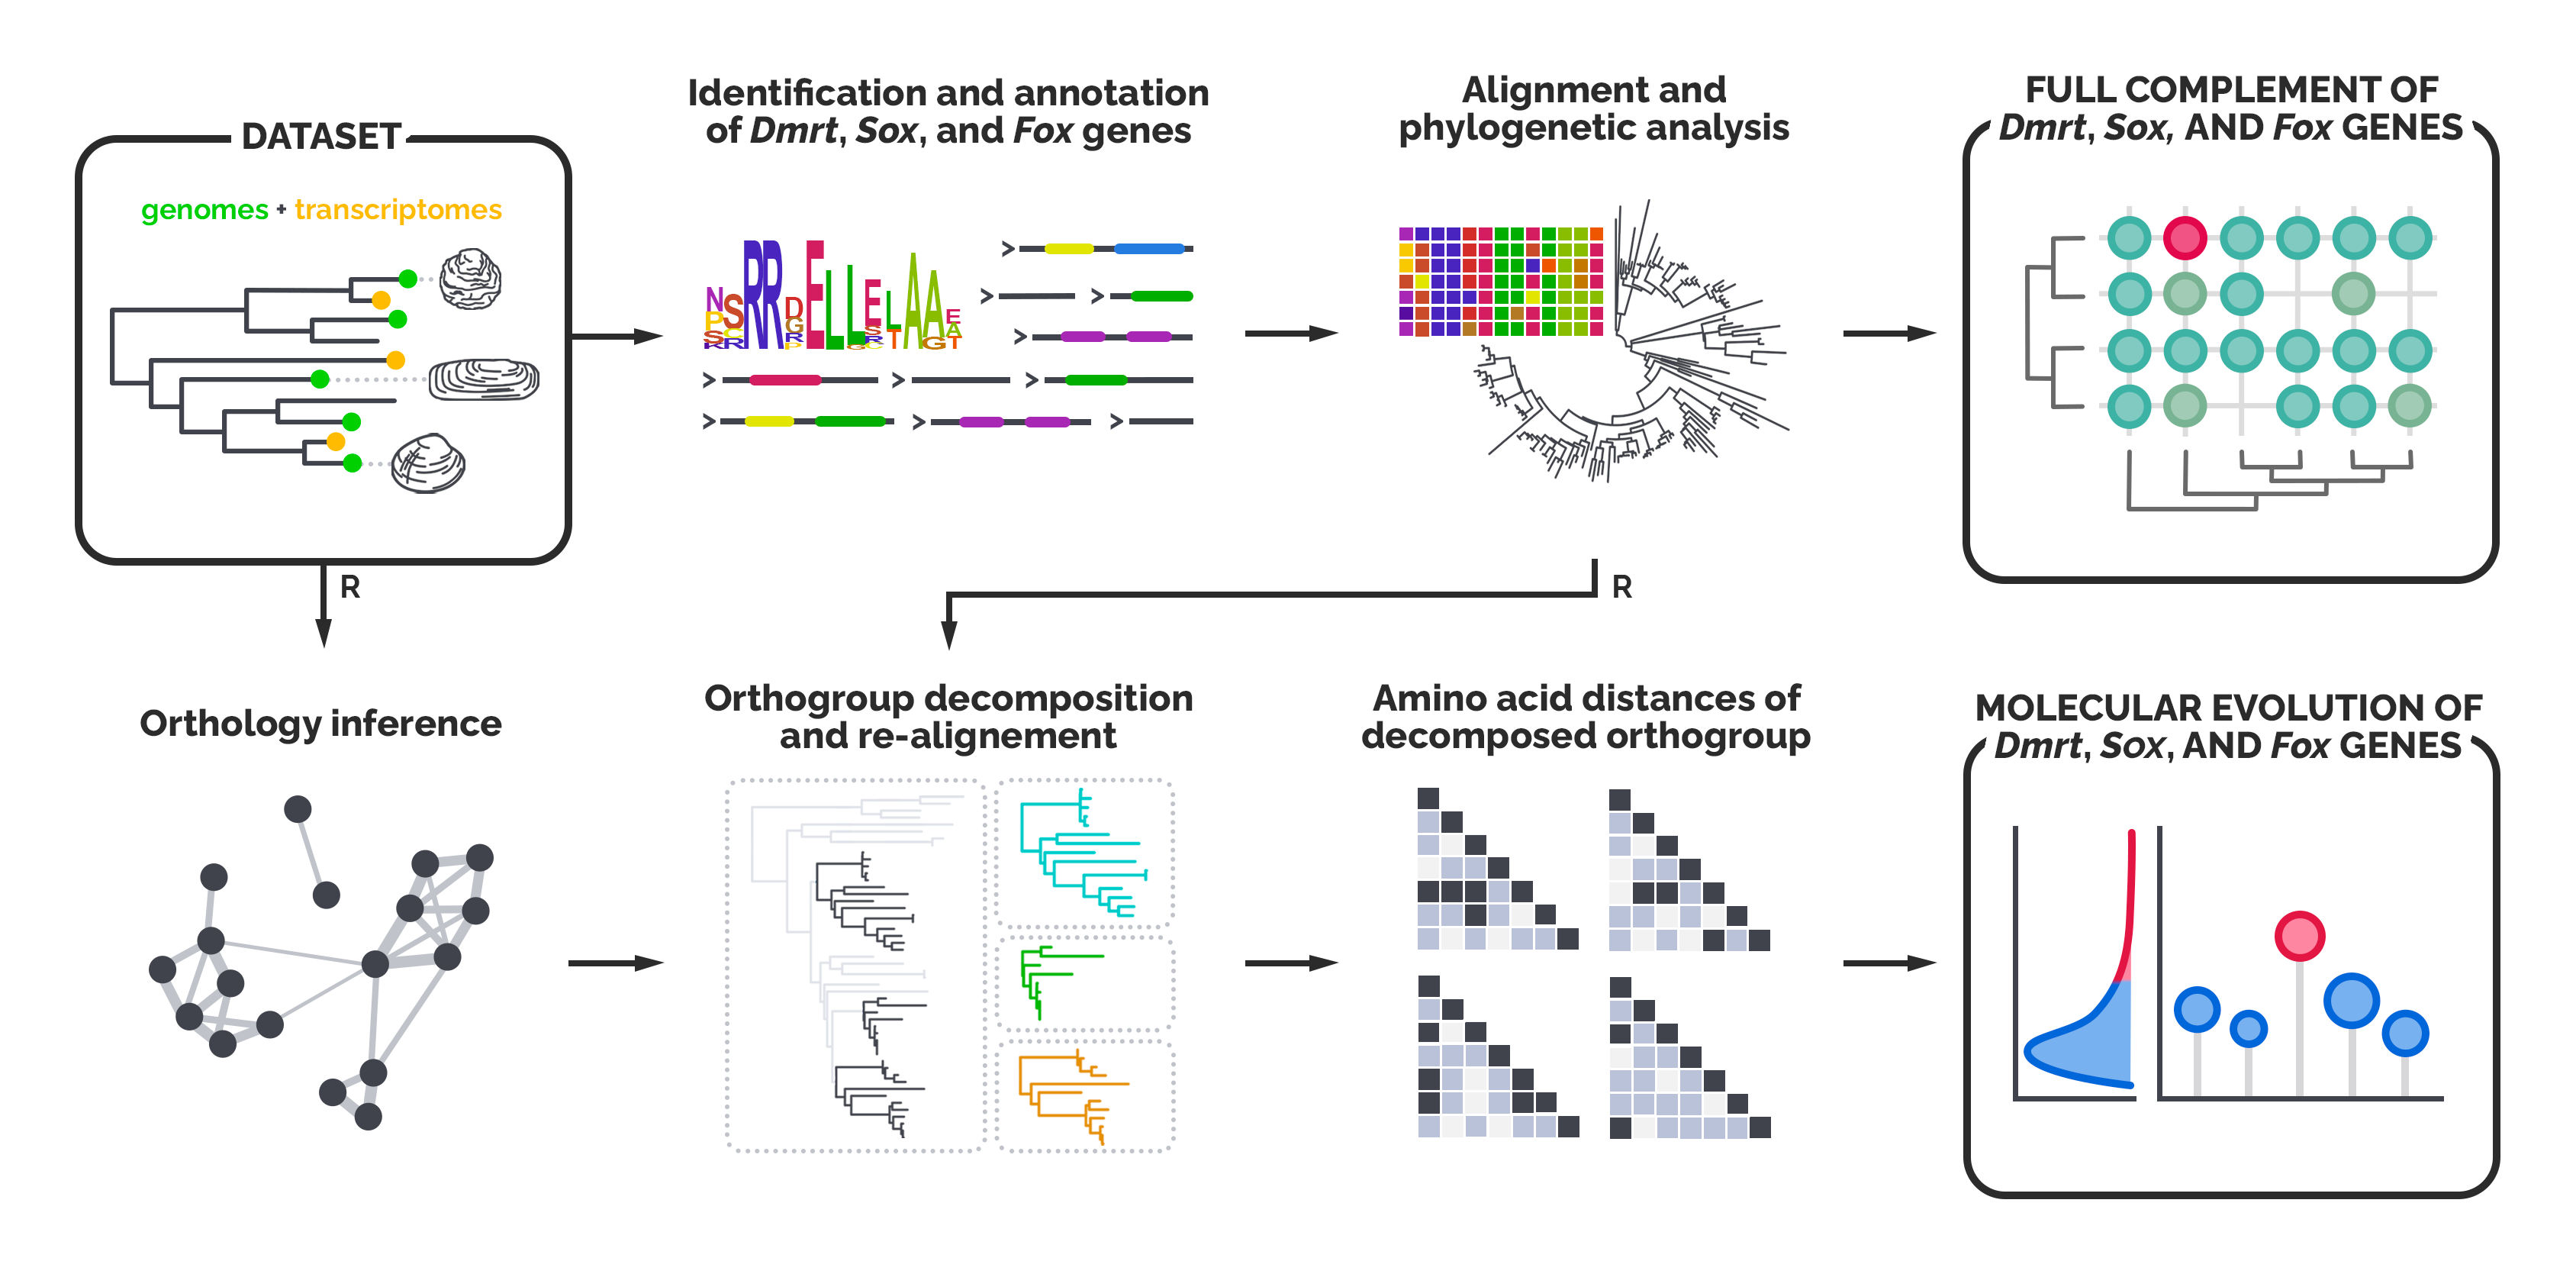
\includegraphics[width=0.9\textwidth]{chapter2/figure_1.png}
	
	\caption[\textbf{Graphical summary of the available knowledge and experiments concerning the genetic basis of \gls{sd} in bivalves, at the level of major taxonomic orders (as reported in WoRMS; accessed before or on 14/03/2023)}]
	{
		\textbf{Graphical summary of the available knowledge and experiments concerning the genetic basis of \gls{sd} in bivalves, at the level of major taxonomic orders (as reported in WoRMS; accessed before or on 14/03/2023)}. For each bivalve clade it is reported: (i) the availability of records of \gls{esd} (ii) the availability of \gls{dge} experiments specifically intended to investigate sex-biased or sex-specific genes; (iii) whether the \gls{dui} of mitochondria has been reported in at least one species; (iv) whether \glspl{hosc} have been identified in at least one species; (v) the availability of \gls{rnai} experiments for genes belonging to the Dmrt, Sox, and Fox gene families. The phylogenetic tree on the left has been drawn on the basis of the most widely accepted topology for bivalves, according to analyses based on nuclear markers and morphological data. The tips of the tree correspond to major bivalve orders, except for Opponobranchia and Anomalodesmata, which represent higher-level taxonomic ranks. References for the availability of data and experiments can be found throughout the main test.
	}
	\label{fig:summarySex}
\end{figure}

Clearly, if a functional interplay between \gls{dui} and \gls{sd} in bivalves is proven, this will provide new research questions regarding not only bivalve biology itself but also broader evolutionary topics (e.g., are there any converging trait between \gls{dui} and \gls{cms} systems? What is the degree of plasticity of such mitochondria-related \gls{sd} systems? Are mitochondria-related \gls{sd} systems more widespread in eukaryotes than currently thought?).

\subsection{Evolution of sex-determination related genes}
Considering this intricate scenario of \gls{sd} mechanisms and the wide diversity of bivalves, in the last years many differential transcription analyses have been performed on several species with the attempt to identify the most probable \glspl{srg} (e.g., \textbf{\cite{milani2013nuclear,zhang2014genomic,chen2017transcriptome,capt2018deciphering,shi2018proteome}}; \cref{fig:summarySex}). Interestingly, certain genes consistently emerged across different bivalve species as being substantially more transcribed in one sex (sex-biased) or exclusively transcribed in one sex (sex-specific), suggesting their potential involvement in the \gls{sd} pathway. These genes mainly belong to the \gls{dmrt}, \gls{sox}, and \gls{fox} families, which play a role in various developmental processes (including the \gls{sd} cascade) in most animals (\textbf{\cite{marshall2010homologies,bachtrog2014sex,beukeboom2014evolution}}). Members of these three gene families are also included in the working model for the \gls{sd} regulatory network proposed for the Pacific oyster \gls{cgig} by \textbf{\cite{zhang2014genomic}}, in which: \textit{CgSoxH} (which belong to the \gls{sox} family) promotes male gonad development by activating \textit{CgDsx} (which belong to the \gls{dmrt} family) and inhibiting \textit{CgFoxL2} (which belong to the \gls{fox} family); \textit{CgFoxL2}, when not inhibited by the pair \textit{CgSoxH}/\textit{CgDsx}, promotes female gonad development. Similarly, \textbf{\cite{han2022ancient}} appointed \textit{FoxL2} as a putative \gls{sd} gene in the two scallop species \gls{pyes} and \gls{cfar}.
If their pivotal role in \gls{sd} of bivalves is confirmed, an evolutionary genomic analysis may help in better understanding why members of the above-mentioned gene families appear particularly prone to be recruited in the \gls{sd} cascade also in distantly related species, as it is observed for \textit{Dmrt1} and \textit{Sox3} homologs in vertebrates (\textbf{\cite{marshall2010homologies,bachtrog2014sex}}; and the following section). Furthermore, considering the occurrence of mixed \gls{sd} systems in bivalves, \gls{dmrt}, \gls{sox}, and \gls{fox} genes may provide new perspectives on the influence of different environmental cues on the molecular evolution of animal \glspl{srg}. However, to date, experiments have been limited to molecular cloning, differential transcription, and tissue localization of such genes (\textbf{\cite{liang2019sox2,sun2022examination}}), while only a few have directly investigated their biological functions in bivalves, for example through post-transcriptional silencing of target mRNAs [\gls{rnai}; \cref{fig:summarySex}; e.g., \textbf{\cite{liang2019sox2,wang2020identification,sun2022examination}}].

Overall, \gls{dmrt}, \gls{sox}, and \gls{fox} genes are highly interesting targets to be investigated in the framework of bivalve \gls{sd} and have indeed obtained much more attention than the study of \glspl{sc} or the role of environmental cues. However, much work is still to be done in order to understand their function in the \gls{sd} signaling pathway and their evolutionary history.

\section{The case of the Dmrt gene family in bivalves}

Among the \gls{srg} candidates identified in bivalves, \gls{dmrt} genes (named after \gls{dsx} from \gls{dmel} and \gls{mab-3} from \gls{cele}) are of particular interest. As a matter of fact, in vertebrates, besides their role in placode neurogenesis and somite patterning (reviewed in \textbf{\cite{mawaribuchi2019independent}}), \gls{dmrt} genes are also involved in the development of male gonads and the maintenance of the testicular function (\textbf{\cite{sun2022examination}}). Their role in the specification and organization of male sexual characters seems indeed to be common across Metazoa, suggesting that a similar function may have been already present in the Bilateria common ancestor (\textbf{\cite{kopp2012dmrt, beukeboom2014evolution}}).

The first attempts to dig inside the phylogenetic history and diversity of bivalve \gls{dmrt} genes have been provided by \textbf{\cite{li2018foxl2}} and \textbf{\cite{evensen2022comparative}}: besides retrieving all the canonical genes (i.e., \textit{Dmrt2}, \textit{Dmrt3} and \textit{Dmrt4/5}), their inferences brought to light a monophyletic \gls{dmrt} group (named \gls{dmrt-1l}) which appears to be private to molluscs and present in several bivalve species. The \gls{dmrt-1l} monophyletic group is confirmed also when expanding the analysis by mining genomes from a wider range of bivalve taxa (\cref{tab:genomes,fig:dmrt-A}), suggesting that \gls{dmrt-1l} genes are widespread in bivalves and were likely present in their common ancestor (\textbf{\cite{evensen2022comparative}}). In particular, \gls{dmrt-1l} genes can been successfully retrieved in species of the orders Mytilida, Ostreida, Pectinida, Unionida, and from \gls{sbro} (Arcida), while the opposite holds for Venerida, \gls{scon} (Adapedonta), and \textit{Dreissena} spp. (Myida; \cref{fig:dmrt-B}). Clearly, the absence of \gls{dmrt-1l} genes demands further investigations, as it may derive from errors in genome assembly and annotations.

\begin{figure}[ht!]
	\centering
	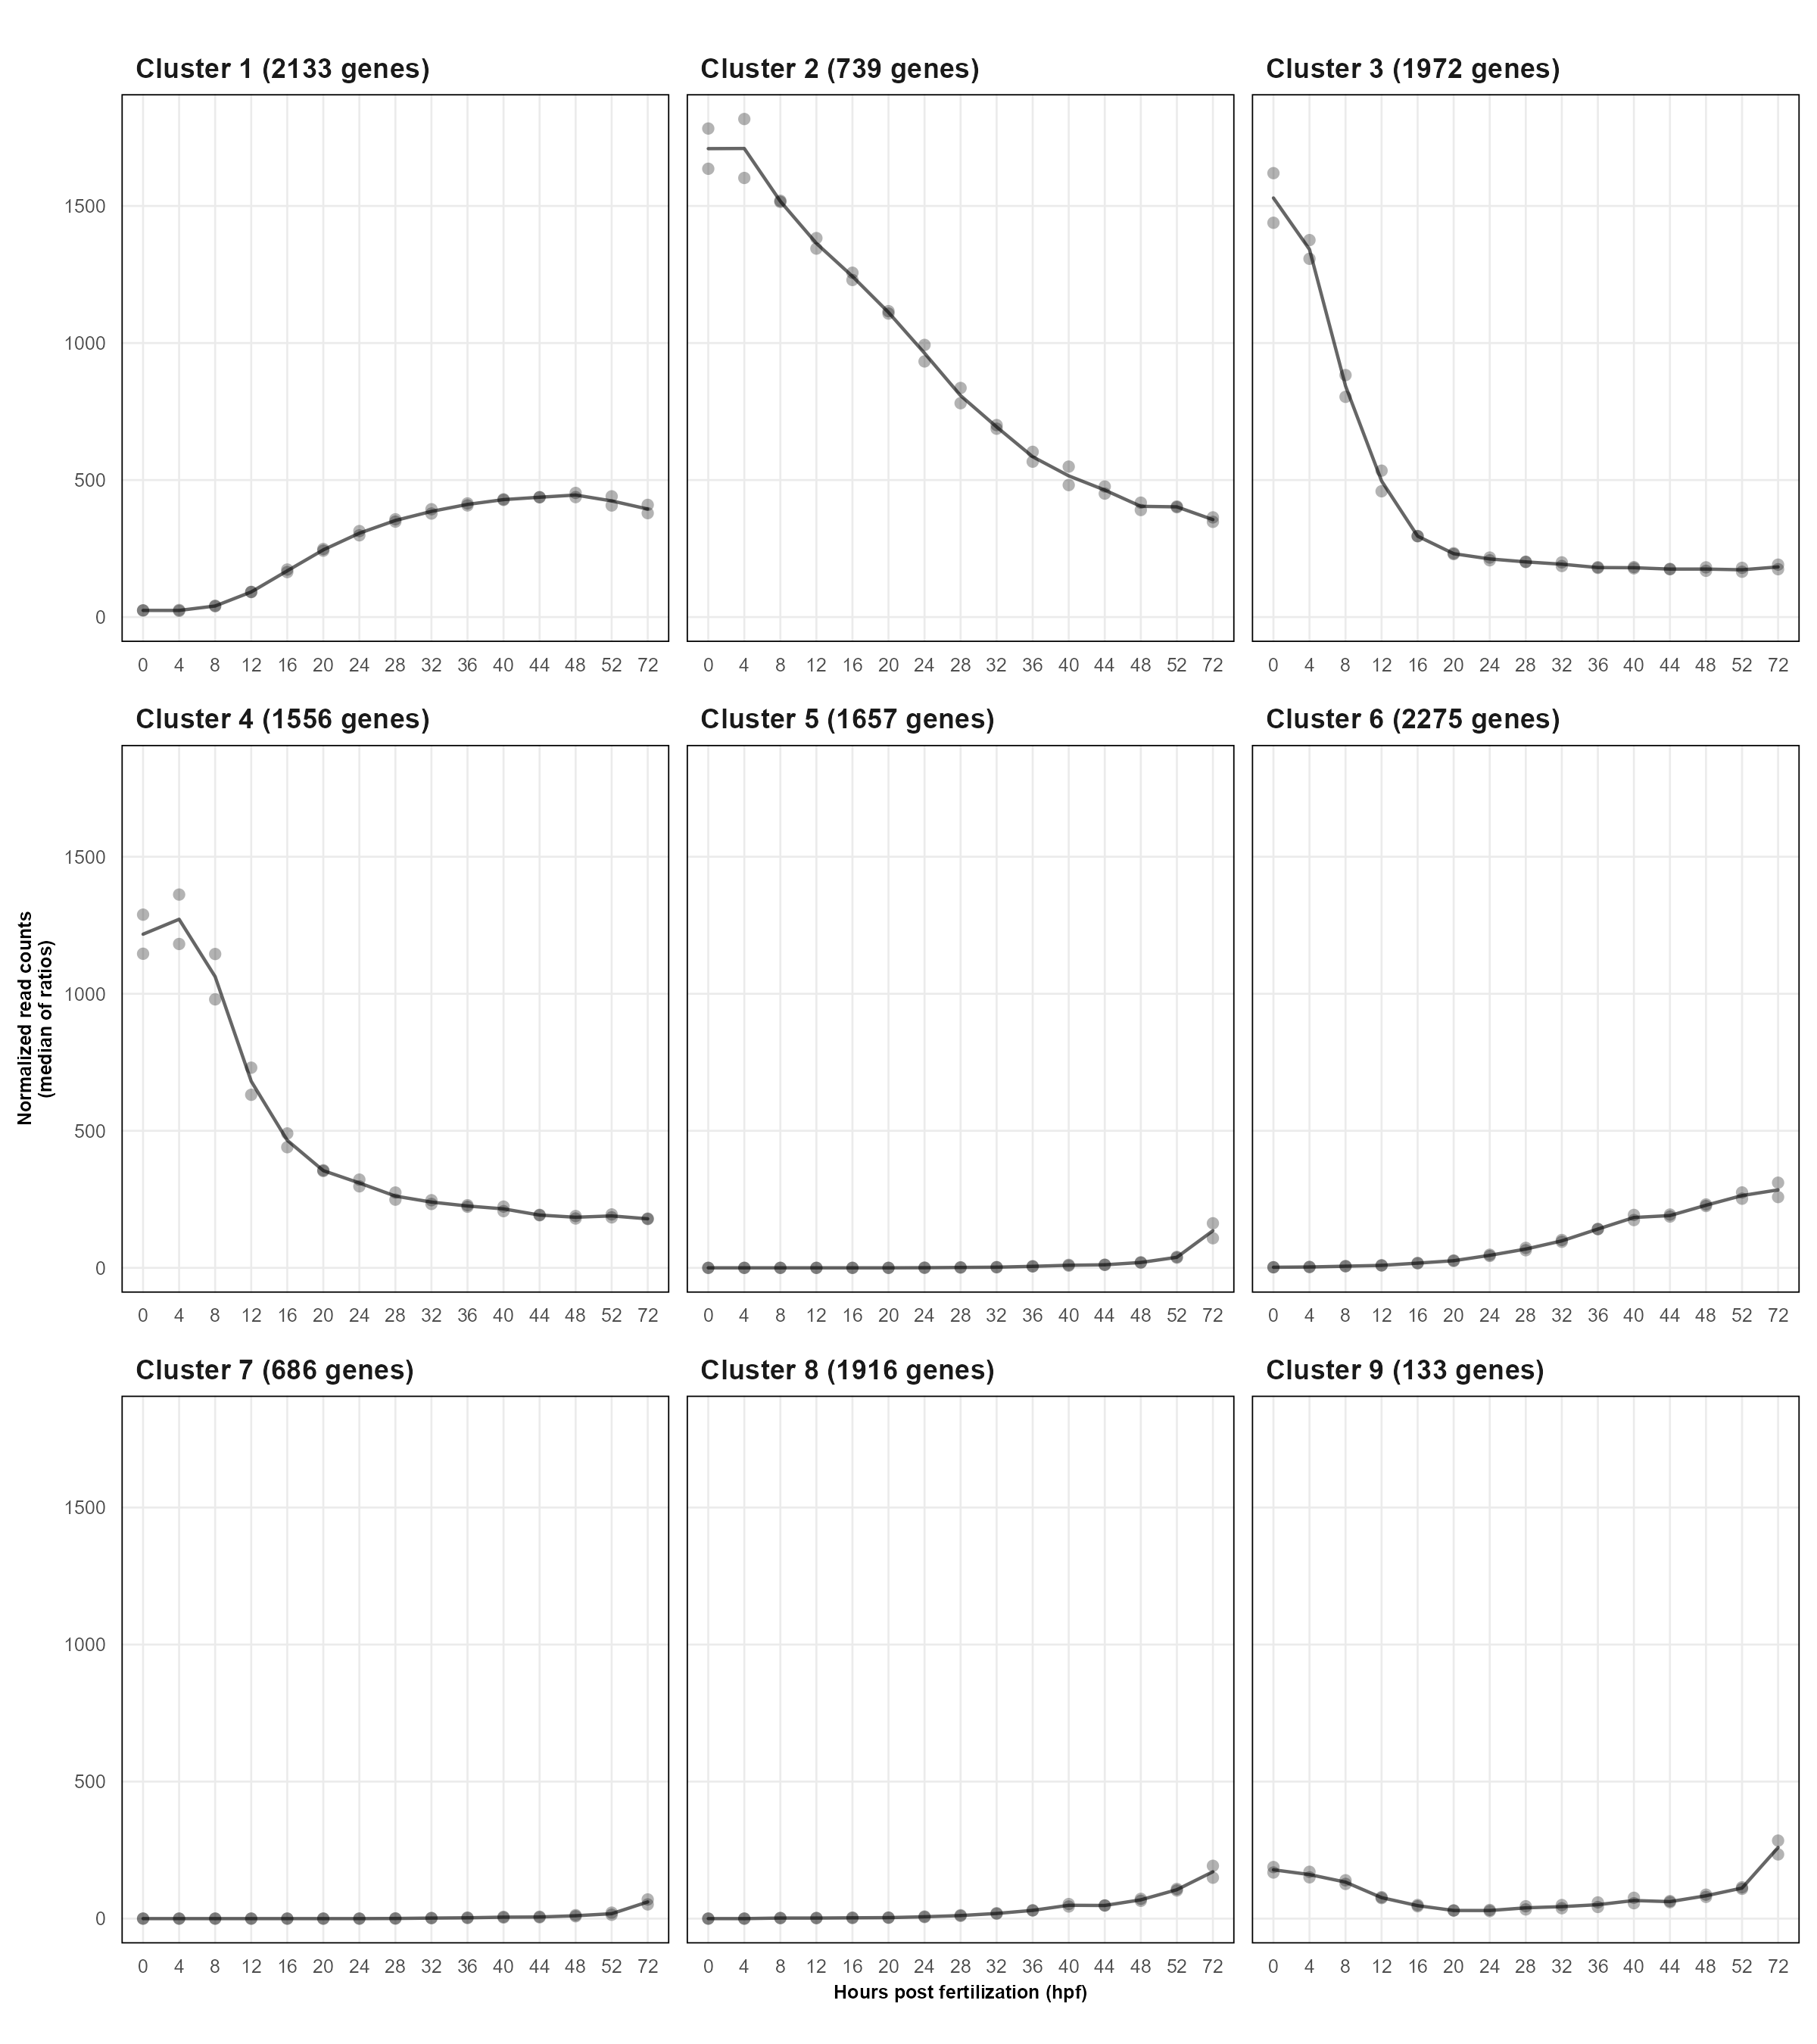
\includegraphics[width=0.9\textwidth]{chapter2/figure_2.png}
	\captionsetup[subfigure]{labelformat=nocaption}
	\begin{subfigure}{0\linewidth}
	\caption{}\label{fig:dmrt-A}
	\end{subfigure}% <----- get rid of space, for proper centering
	\begin{subfigure}{0\linewidth}
	\caption{}\label{fig:dmrt-B}
	\end{subfigure}% <----- get rid of space, for proper centering
	\begin{subfigure}{0\linewidth}
	\caption{}\label{fig:dmrt-C}
	\end{subfigure}% <----- get rid of space, for proper centering
	
	\caption[\textbf{Phylogenetic tree (A) and taxonomic distribution (B) of Dmrt genes in bivalves, and comparison of amino acid pairwise distances within \textit{Dmrt-1L} and the other Dmrts (B)}]
	{
		\textbf{Phylogenetic tree (A) and taxonomic distribution (B) of Dmrt genes in bivalves, and comparison of amino acid pairwise distances within \textit{Dmrt-1L} and the other Dmrts (C)}. (A) Dmrt orthologs from bivalve genome assemblies were obtained with HMMsearch (HMMER toolkit; \textbf{\cite{eddy2011accelerated}}) with the Pfam HMM profile of the DM domain (PF00751). Amino acid alignment was obtained with MAFFT-DASH (\textbf{\cite{rozewicki2019mafft}}), and manually inspected to remove poorly aligning sequences, and trimmed with trimAl (gap threshold of 60\%; \textbf{\cite{capella2009trimal}}). The phylogenetic analysis was carried out using IQ-TREE 2 (\textbf{\cite{minh2020iq}}) with default parameters. Nodes with bootstrap values greater than 84 are marked with filled black circles. The tree was rooted according to \textbf{\cite{evensen2022comparative}}. Dmrt genes analysed by \textbf{\cite{evensen2022comparative}} were used as reference to annotate the various orthology groups, and accession numbers are reported in the tree. The phylogenetic tree with all annotated tips and nodes can be accessed on supplementary material online. (B) Taxonomic distribution of identified Dmrt genes in bivalve genomes. Orders as reported in WoRMS (accessed before or on 14/03/2023) and in \cref{fig:summarySex} are specified. (C) Pairwise amino acid distances were computed for amino acid sequences within each Dmrt orthology group identified in the tree, with the R package ‘phangorn’ (\textbf{\cite{schliep2011phangorn}}) under the JTT substitution model. After checking for normality with the Shapiro-Wilk test ($W = 0.88544$, $p-value < \num{2.2e-16}$) and for group effect with the Kruskal-Wallis test ($p < \num{2.2e-16}$), the pairwise Wilcoxon rank-sum test was used to compare the distributions of pairwise amino acid distances of Dmrt-1L and the other Dmrts. Horizontal bars mark the significative results with $p < 2.2e-16$ (‘****’) (Bonferroni correction for multiple test was applied). The list of genome assemblies used for these analyses and species identifiers can be found in \cref{tab:genomes}. Un.: Unionida; Ad.: Adapedonta; My.: Myida; Ar.: Arcida.
	}

	\label{fig:dmrt}
\end{figure}

The present analysis also supports a higher amino acid sequence divergence of the \gls{dmrt-1l} orthology group with respect to the other \gls{dmrt} orthology groups (\cref{fig:dmrt-C}), which may be explained by a higher rate of sequence evolution related to their sex-biased expression in certain species (\textbf{\cite{zhang2014genomic,shi2015novo,li2018foxl2,evensen2022comparative}}). This is consistent with what has been already observed for the \glspl{srg} \textit{Dmrt1} and \gls{dsx} in vertebrates and \textit{Drosophila}, respectively (e.g., \textbf{\cite{bewick2011evolution,baral2019genetic}}). In fact, sex-biased genes (including \glspl{srg}) often tend to evolve faster than unbiased genes at the level of protein sequences, either when considering male-biased (reviewed in \textbf{\cite{parsch2013evolutionary,grath2016sex}}) or female-biased genes (e.g., \textbf{\cite{papa2017anopheles,ghiselli2018comparative}}). Another possible explanation for the higher amino acid divergence of \gls{dmrt-1l} genes may lie on their expression breadth, that is, genes with a narrow tissue-specific expression tend to evolve faster than more ubiquitous genes (\textbf{\cite{parsch2013evolutionary,xu2022multi}}). As a matter of fact, \gls{dmrt-1l} genes have been found to be significantly more transcribed in the gonadic tissue (particularly in testes) in \gls{pyes} (\textbf{\cite{li2018foxl2}}) and \gls{cgig} (\textbf{\cite{yue2021variance}}).

Understanding the role and molecular interactions of \gls{dmrt-1l} genes in bivalve \gls{sd} and gonad development would greatly enhance the possibility of outlining the evolutionary causes and consequences of their high amino acid divergence (\cref{fig:dmrt-C}), for example by linking the molecular evolution to the degree of pleiotropy. However, most of our knowledge on \gls{dmrt-1l} biology is currently limited to the temporal and tissue localization of transcripts in a few species of bivalves (e.g., \textbf{\cite{li2018foxl2,yue2021variance}}). In fact—apart from the work by \textbf{\cite{sun2022examination}}, which confirmed the role of \gls{dmrt-1l} in the gonad development of \gls{cgig} through non-invasive \gls{rnai} and found that the knocked-down phenotype results in size reduction of male gonads—no other experiments intended to elucidate the function of \gls{dmrt-1l} genes in bivalves have been carried out so far (\cref{fig:summarySex}). This clearly hinders any possible integration between molecular data with functional assays.
If the role of \gls{dmrt-1l} as major sex determinants was confirmed, bivalves would become an intriguing clade in which investigate why, in Metazoa, certain genes (namely, the \gls{dmrt} gene family) appear particularly prone to being recruited at the top of the \gls{sd} cascade. To date, this phenomenon has been widely examined in vertebrates, where \textit{Dmrt1} genes have independently gained a primary role in male \gls{sd} in fish, amphibians, and birds, and are considered candidate sex-determining genes also in monotreme mammals (\textbf{\cite{marshall2010homologies,beukeboom2014evolution,mawaribuchi2019independent}}). Bivalves may provide an alternative evolutionary scenario to study the selective forces and molecular modifications that support \gls{dmrt} genes in repeatedly taking over the \gls{sd} process. In fact, since \gls{dmrt-1l} genes seem to be restricted to molluscs (\cref{fig:dmrt-A}), it would be intriguing to clarify if the putative involvement in the \gls{sd} cascade of extant bivalve species is the result of shared ancestry or convergent evolution, which would establish a study system for the evolution of \gls{dmrt} genes parallel to that of vertebrates (see \textbf{\cite{capel2017vertebrate}}).

Obviously, \gls{dmrt-1l} should not be expected to be the sole sex-determining gene. In fact, \textit{Fox-L2} has already been appointed as the female sex-determining gene in \gls{pyes} and \gls{cfar} (\textbf{\cite{han2022ancient}}). Consequently, we should expect that other primary genetic determinants exist, consistently with the extremely high species diversity of the clade. Thus, bivalves may additionally serve as a valuable model system to study how genes from different families take over the \gls{sd} cascade and are shaped by selection.

\section{Conclusions: bivalves as new models in the study of sex determination}
\gls{sd} is undoubtedly a fascinating biological and evolutionary topic as much as it is challenging to investigate. Our understanding of the causes and consequences of the \gls{sd} mechanism diversity strongly relies on the study of different systems and non-model model organisms (\textbf{\cite{bachtrog2014sex,milani2020faraway}}), which provide the foundation for depicting a comprehensive evolutionary and comparative framework in which new and coherent research perspectives can be grounded.

In recent years, bivalves have been achieving growing importance in many fields of biology, from ecology to genomics, and from environmental biomonitoring to mitochondrial studies (\textbf{\cite{milani2020faraway,ghiselli2021bivalve}}), but they can be a valuable model to address also \gls{sd} studies. The diversity of their life history traits provides indeed a challenging, yet extremely fascinating framework, to put the \gls{sd} processes into an evolutionary context.

Bivalves can help us explain how \gls{esd} and \gls{gsd} interplay with each other in response to the environmental conditions, as a mixed system of both has been proposed to act in the establishment of bivalve sexual identity (reviewed in \textbf{\cite{breton2018sex}}). Moreover, the occurrence of the many existing variants of hermaphroditism and gonochorism even in closely related species, or within the same population, strongly suggests that the basic \gls{sd} pathway (whether genetic, environmental, or mixed) should be plastic enough to sustain the existence of individuals of both sexes, thus providing the opportunity to study how \gls{sd} gene regulatory networks are shaped and selected throughout evolution and how epigenetic regulation may influence SD. The unique DUI system further poses an undeniable challenge in \gls{sd} studies since it may represent an \gls{sd}-linked mechanism which relies on the non-nuclear portion of the genome and may unfold many new research paths (\textbf{\cite{milani2020faraway,ghiselli2021bivalve}}). Nonetheless, much of the research effort on bivalve \gls{sd} has been devolved to specific groups of socio-economic importance, such as Mytilida, Ostreida, Pectinida, and Unionida, while the other lineages of the bivalve phylogeny have been neglected (\cref{fig:summarySex}). Our understanding of the \gls{sd} processes of bivalves is thus restricted and is mainly lacking a broad comparative framework in which to draw comprehensive evolutionary inferences.

Genes from the \gls{dmrt}, \gls{sox} and \gls{fox} families, which are involved in \gls{sd} also in other Metazoa, may be considered excellent genomic targets to study the processes and patterns of molecular evolution in sex-biased genes, as well as of the recurrent recruitment of genes in the \gls{sd} cascade. Also, identifying the major genetic regulators of \gls{sd} in bivalves would burst the functional study of the interaction between \gls{esd} and GSD, by providing genetic targets that can be manipulated through \gls{rnai} and/or genome editing techniques to understand the role of environmental cues in SD. In the same way, knowing the main genetic actors of \gls{sd} would allow researcher to identify \glspl{sc} not only on the basis of in-silico techniques (such as k-mer based or SNP methods) but also by less-expensive wet lab protocols (such as fluorescence \gls{ish} on metaphase chromosome plates). Furthermore, it would help to understand whether and how the mitochondrial additional \glspl{orf} of \gls{dui} species interact with the \gls{sd} system, by performing thorough gene expression essays.

In conclusion, we strongly urge researchers to invest more resources in the integrative study of bivalve \gls{sd} to unravel the many underlying mechanisms and expand our understanding of this biological process. Given our limited knowledge in the field, one of the first routes that should be undertaken may rely on the comparative study of \glspl{srg} of bivalves from a genomic perspective, as this kind of data is nowadays growing at a rate faster than ever. Establishing such a genomic ground plan for understudied organisms will in fact allow researchers to develop evolutionary-aware experiments with better selected genetic targets.

\begin{landscape}
	\footnotesize
	\begin{longtable}[c]{@{}lllllll@{}}
		\caption[\textbf{List of bivalve genomes from which Dmrt genes have been extracted}]
		{
			\textbf{List of bivalve genomes from which Dmrt genes have been extracted}. For each species, the accepted name and the most-common synonym (in parentheses) are reported. NCBI accession numbers are provided, when available, as well as BUSCO scores of the predicted proteomes against the ‘metazoa\_odb10’ dataset (\textbf{\cite{manni2021busco}}).
		}
		\label{tab:genomes}                                                                               \\
		\toprule
		\textbf{Species}                                                                                &
		\textbf{ID}                                                                                     &
		\textbf{Order}                                                                                  &
		\textbf{Assembly level}                                                                         &
		\textbf{BUSCO score}                                                                            &
		\textbf{Reference}                                                                              &
		\textbf{NCBI Acc. No.}                                                                            \\* \hline \hline
		\endfirsthead
		%
		\multicolumn{7}{c}%
		{\textbf{Tab. \thetable}\ continued from previous page}                                       \\
		\toprule
		\textbf{Species}                                                                                &
		\textbf{ID}                                                                                     &
		\textbf{Order}                                                                                  &
		\textbf{Assembly level}                                                                         &
		\textbf{BUSCO score}                                                                            &
		\textbf{Reference}                                                                              &
		\textbf{NCBI Acc. No.}                                                                            \\* \hline \hline
		\endhead
		%
		\endfoot
		%
		\endlastfoot
		%
		\textit{Anadara (Scapharca) broughtonii}                                                        &
		Sbro                                                                                            &
		Arcida                                                                                          &
		Chromosome                                                                                      &
		\begin{tabular}[c]{@{}l@{}}C:91.2\%\\ {[}S:85.6\%,D:5.6\%{]}\\ F:2.6\%\\ M:6.2\%\end{tabular}   &
		\textbf{\cite{bai2019chromosomal}}                                                              &
		NA                                                                                                \\* \midrule
		\textit{Sinonovacula constricta}                                                                &
		Scon                                                                                            &
		Adapedonta                                                                                      &
		Chromosome                                                                                      &
		\begin{tabular}[c]{@{}l@{}}C:92.5\%\\ {[}S:80.4\%,D:12.1\%{]}\\ F:3.4\%\\ M:4.1\%\end{tabular}  &
		\textbf{\cite{ran2019chromosome}}                                                               &
		GCA\_007844125.1                                                                                  \\* \midrule
		\textit{Dreissena polymorpha}                                                                   &
		Dpol                                                                                            &
		Myida                                                                                           &
		Chromosome                                                                                      &
		\begin{tabular}[c]{@{}l@{}}C:86.9\%\\ {[}S:75.1\%,D:11.8\%{]}\\ F:6.4\%\\ M:6.7\%\end{tabular}  &
		\textbf{\cite{mccartney2022genome}}                                                             &
		GCA\_020536995.1                                                                                  \\* \midrule
		\textit{Dreissena rostriformis}                                                                 &
		Dros                                                                                            &
		Myida                                                                                           &
		Scaffold                                                                                        &
		\begin{tabular}[c]{@{}l@{}}C:75.2\%\\ {[}S:73.2\%,D:2.0\%{]}\\ F:15.2\%\\ M:9.6\%\end{tabular}  &
		\textbf{\cite{calcino2019quagga}}                                                               &
		GCA\_007657795.1                                                                                  \\* \midrule
		\textit{Mytilus unguiculatus (coruscus)}                                                        &
		Mcor                                                                                            &
		Mytilida                                                                                        &
		Chromosome                                                                                      &
		\begin{tabular}[c]{@{}l@{}}C:80.0\%\\ {[}S:79.1\%,D:0.9\%{]}\\ F:7.7\%\\ M:12.3\%\end{tabular}  &
		\textbf{\cite{yang2021chromosome}}                                                              &
		GCA\_017311375.1                                                                                  \\* \midrule
		\textit{Mytilus edulis}                                                                         &
		Medu                                                                                            &
		Mytilida                                                                                        &
		Scaffold                                                                                        &
		\begin{tabular}[c]{@{}l@{}}C:83.7\%\\ {[}S:64.5\%,D:19.2\%{]}\\ F:5.2\%\\ M:11.1\%\end{tabular} &
		\textbf{\cite{corrochano2022evidence}}                                                          &
		GCA\_905397895.1                                                                                  \\* \midrule
		\textit{Mytilus galloprovincialis}                                                              &
		Mgal                                                                                            &
		Mytilida                                                                                        &
		Scaffold                                                                                        &
		\begin{tabular}[c]{@{}l@{}}C:80.3\%\\ {[}S:47.5\%,D:32.8\%{]}\\ F:8.8\%\\ M:10.9\%\end{tabular} &
		\textbf{\cite{gerdol2020massive}}                                                               &
		GCA\_900618805.1                                                                                  \\* \midrule
		\textit{Perna viridis}                                                                          &
		Pvir                                                                                            &
		Mytilida                                                                                        &
		Scaffold                                                                                        &
		\begin{tabular}[c]{@{}l@{}}C:99.4\%\\ {[}S:99.0\%,D:0.4\%{]}\\ F:0.2\%\\ M:0.4\%\end{tabular}   &
		\textbf{\cite{inoue2021genomics}}                                                               &
		GCA\_018327765.1                                                                                  \\* \midrule
		\textit{Magallana (Crassostrea) ariakensis}                                                     &
		Cari                                                                                            &
		Ostreida                                                                                        &
		Chromosome                                                                                      &
		\begin{tabular}[c]{@{}l@{}}C:94.6\%\\ {[}S:90.9\%,D:3.7\%{]}\\ F:0.9\%\\ M:4.5\%\end{tabular}   &
		\textbf{\cite{li2021genome}}                                                                    &
		GCA\_020567875.1                                                                                  \\* \midrule
		\textit{Magallana (Crassostrea) gigas}                                                          &
		Cgig                                                                                            &
		Ostreida                                                                                        &
		Chromosome                                                                                      &
		\begin{tabular}[c]{@{}l@{}}C:98.5\%\\ {[}S:67.6\%,D:30.9\%{]}\\ F:0.3\%\\ M:1.2\%\end{tabular}  &
		\textbf{\cite{penaloza2021chromosome}}                                                          &
		GCF\_902806645.1                                                                                  \\* \midrule
		\textit{Crassostrea virginica}                                                                  &
		Cvir                                                                                            &
		Ostreida                                                                                        &
		Chromosome                                                                                      &
		\begin{tabular}[c]{@{}l@{}}C:98.1\%\\ {[}S:58.6\%,D:39.5\%{]}\\ F:0.3\%\\ M:1.6\%\end{tabular}  &
		\textbf{\cite{gomez2015developing}}                                                             &
		GCF\_002022765.2                                                                                  \\* \midrule
		\textit{Saccostrea glomerata}                                                                   &
		Sglo                                                                                            &
		Ostreida                                                                                        &
		Scaffold                                                                                        &
		\begin{tabular}[c]{@{}l@{}}C:88.9\%\\ {[}S:85.3\%,D:3.6\%{]}\\ F:5.1\%\\ M:6.0\%\end{tabular}   &
		\textbf{\cite{powell2018genome}}                                                                &
		GCA\_003671525.1                                                                                  \\* \midrule
		\textit{Argopecten irradians concentricus}                                                      &
		Airc                                                                                            &
		Pectinida                                                                                       &
		Scaffold                                                                                        &
		\begin{tabular}[c]{@{}l@{}}C:94.8\%\\ {[}S:93.9\%,D:0.9\%{]}\\ F:3.7\%\\ M:1.5\%\end{tabular}   &
		\textbf{\cite{liu2020draft}}                                                                    &
		GCA\_004382765.1                                                                                  \\* \midrule
		\textit{Argopecten irradians irradians}                                                         &
		Airi                                                                                            &
		Pectinida                                                                                       &
		Scaffold                                                                                        &
		\begin{tabular}[c]{@{}l@{}}C:94.8\%\\ {[}S:93.9\%,D:0.9\%{]}\\ F:3.7\%\\ M:1.5\%\end{tabular}   &
		Liu et al., 2020                                                                                &
		GCA\_004382745.1                                                                                  \\* \midrule
		\textit{Argopecten purpuratus}                                                                  &
		Apur                                                                                            &
		Pectinida                                                                                       &
		Scaffold                                                                                        &
		\begin{tabular}[c]{@{}l@{}}C:89.2\%\\ {[}S:88.5\%,D:0.7\%{]}\\ F:5.0\%\\ M:5.8\%\end{tabular}   &
		\textbf{\cite{liu2020draft}}
		NA                                                                                                \\* \midrule
		\textit{Pecten maximus}                                                                         &
		Pmax                                                                                            &
		Pectinida                                                                                       &
		Chromosome                                                                                      &
		\begin{tabular}[c]{@{}l@{}}C:98.5\%\\ {[}S:74.7\%,D:23.8\%{]}\\ F:0.4\%\\ M:1.1\%\end{tabular}  &
		\textbf{\cite{kenny2020gene}}                                                                   &
		GCF\_902652985.1                                                                                  \\* \midrule
		\textit{Mizuhopecten (Patinopecten) yessoensis}                                                 &
		Pyes                                                                                            &
		Pectinida                                                                                       &
		Scaffold                                                                                        &
		\begin{tabular}[c]{@{}l@{}}C:98.6\%\\ {[}S:75.2\%,D:23.4\%{]}\\ F:0.4\%\\ M:1.0\%\end{tabular}  &
		\textbf{\cite{wang2017scallop}}                                                                 &
		GCF\_002113885.1                                                                                  \\* \midrule
		\textit{Margaritifera margaritifera}                                                            &
		Mmar                                                                                            &
		Unionida                                                                                        &
		Scaffold                                                                                        &
		\begin{tabular}[c]{@{}l@{}}C:92.6\%\\ S:82.3\%,D:10.3\%{]}\\ F:3.2\%\\ M:4.2\%\end{tabular}     &
		\textbf{\cite{gomes2021crown}}                                                                  &
		GCA\_015947965.1                                                                                  \\* \midrule
		\textit{Potamilus streckersoni}                                                                 &
		Pstr                                                                                            &
		Unionida                                                                                        &
		Scaffold                                                                                        &
		\begin{tabular}[c]{@{}l@{}}C:74.7\%\\ {[}S:73.8\%,D:0.9\%{]}\\ F:7.0\%\\ M:18.3\%\end{tabular}  &
		\textbf{\cite{smith2021high}}                                                                   &
		GCA\_016746295.1                                                                                  \\* \midrule
		\textit{Calyptogena (Archivesica) marissinica}                                                  &
		Amar                                                                                            &
		Venerida                                                                                        &
		Chromosome                                                                                      &
		\begin{tabular}[c]{@{}l@{}}C:82.0\%\\ {[}S:80.0\%,D:2.0\%{]}\\ F:6.1\%\\ M:11.9\%\end{tabular}  &
		\textbf{\cite{ip2021host}}                                                                      &
		GCA\_014843695.1                                                                                  \\* \midrule
		\textit{Cyclina sinensis}                                                                       &
		Csin                                                                                            &
		Venerida                                                                                        &
		Scaffold                                                                                        &
		\begin{tabular}[c]{@{}l@{}}C:94.0\%\\ {[}S:83.8\%,D:10.2\%{]}\\ F:1.9\%\\ M:4.1\%\end{tabular}  &
		\textbf{\cite{wei2020chromosome}}                                                               &
		GCA\_012932295.1                                                                                  \\* \midrule
		\textit{Mercenaria mercenaria}                                                                  &
		Mmer                                                                                            &
		Venerida                                                                                        &
		Chromosome                                                                                      &
		\begin{tabular}[c]{@{}l@{}}C:95.4\%\\ {[}S:70.9\%,D:24.5\%{]}\\ F:0.5\%\\ M:4.1\%\end{tabular}  &
		\textbf{\cite{song2021hard}}                                                                    &
		GCF\_014805675.1                                                                                  \\* \midrule
		\textit{Ruditapes   philippinarum}                                                              &
		Rphi                                                                                            &
		Venerida                                                                                        &
		Chromosome                                                                                      &
		\begin{tabular}[c]{@{}l@{}}C:83.4\%\\ {[}S:74.5\%,D:8.9\%{]}\\ F:8.8\%\\ M:7.8\%\end{tabular}   &
		\textbf{\cite{xu2022multi}}                                                                     &
		GCA\_026571515.1                                                                                  \\* \bottomrule \bottomrule
	\end{longtable}
\end{landscape}

\section{Acknowledgments}
The authors are extremely thankful to Sofía Blanco González from the University of Vigo for her willingness to engage in discussions and for genuinely sharing her opinion on this work.

\section{Data Availability}
Analyzed data and R scripts used to generate plots can be accessed in supplementary material online deposited at the following GitHub repository: \href{https://github.com/filonico/bivalve_sex_perspective}{filonico/bivalve\_sex\_perspective}.

% \end{document}